\section{Proof for rank 5}

\subsection{Basic results v2}

\begin{proposition}
  If a vertex is linked with three edges that does not share the other end, then two of those three edges are part of an alternating square.
\end{proposition}

\begin{proof}
  Among the three edges, at least two are not adjacent and thus, they need to be part of an alternating square.
\end{proof}

\begin{corollary}
  If an vertex is not part of any alternating square, then it it connected to at most two other vertices.
\end{corollary}

\begin{proposition}
  In a connected CPR graph over more than two vertices, there no triple edge outside of an alternating square and there is no double edge such that the difference between indices is not 2.
\end{proposition}

\begin{proof}
  Each end of the triple edge is not part of an alternating square and so must not be connected to more than 2 vertices. But the graph is connected, so at least one end of the graph must be connected to more than one vertex. So one end must be connected to two vertices but then the edge that connect this vertex to the new one must be adjacent to all three edges. But that is impossible.
\end{proof}

\begin{proposition}
  An alternating square can be connected to a simple edge (no part of an alternating square) only if it have two adjacent simple edges with a difference in indices of exactly 2.
\end{proposition}



\subsection{Basic results}

\paragraph{}
Dans la suite, nous noterons les carrés alternés grâce au deux involutions qui les composent. Un carré alterné avec des arêtes $\rho_0$ et $\rho_2$ sera noté $[\rho_0, \rho_2]$.

\begin{definition}
  Deux carrés alternés sont dit adjacents s'ils partagent deux sommets\footnote{Ces définitions sont à améliorer, il y a quelques problèmes mais je pense qu'il y a moyen de rendre ça correct}.
\end{definition}

\begin{definition}
  Une suite de carrés alternés adjacents est un suite finie dans laquelle chaque carré alterné est adjacent avec son précédesseur et son successeur s'ils existent.
\end{definition}

\begin{definition}
  Une suite de carré alternés adjacents est dite linéaire si une des deux composante de sa notation est constante.
\end{definition}

Par exemple, la suite $[\rho_0, \rho_2], [\rho_0, \rho_4], [\rho_0, \rho_3]$ est linéaire car la première composante est toujours $\rho_0$.

\begin{definition}
  Une suite de carré alterné est dite monotone si la suite formée par les différences des indices de ses carrés est monotone.
\end{definition}

La suite $[\rho_0, \rho_2], [\rho_0, \rho_3], [\rho_0, \rho_4]$ est monotone, en effet la suite formée par la différente des indice est $2, 3, 4$ et cette suite est bien monotone.

\begin{proposition}
  Toute suite de carrés alternés monotone est linéaire.
\end{proposition}

\begin{proof}
  Une suite monotone non-linéaire serait de la forme suivante: $[\rho_{i-1}, \rho_j], [\rho_i, \rho_j], [\rho_i, \rho_{j+1}]$, si nous représentons le graphe d'une telle suite nous obtenons le graphe suivant:

  \begin{figure}[H]
    \begin{center}
      \begin{tikzpicture}

        \begin{scope}[every node/.style={circle,draw}]
          \node (1)  at (0,2)  {};
          \node (2)  at (0,0)  {};
          \node (3)  at (0,-2) {};
          \node (4)  at (2,2)  {};
          \node (5)  at (2,0)  {};
          \node (6)  at (2,-2) {};
          \node (7)  at (4,2)  {};
          \node (8)  at (4,0)  {};
        \end{scope}

        \begin{scope}[every node/.style={fill=white,circle}]

          \begin{scope}[every edge/.style={draw}]
            \path (2)  edge node {$i-1$} (3);
            \path (5)  edge node {$i-1$} (6);
            \path (1)  edge node {$i$} (2);
            \path (4)  edge node {$i$} (5);
            \path (7)  edge node {$i$} (8);
            \path (1)  edge node {$j$} (4);
            \path (2)  edge node {$j$} (5);
            \path (3)  edge node {$j$} (6);
            \path (4)  edge node {$j+1$} (7);
            \path (5)  edge node {$j+1$} (8);
          \end{scope}
        \end{scope}

      \end{tikzpicture}
      \caption{Suite de carrés alternés monotone et non-linéaire}
    \end{center}
  \end{figure}

  \paragraph{}
  Nous avons un problème en bas à droite, nous ne pouvons pas ajouter de carré à cet endroit sinon nous n'avons plus une suite, donc il faut que $i-1$ et $j+1$ soit consécutifs. On a alors $i = j+1$ ou $i+1=j$ étant donné la symétrie nous pouvons n'en conserver qu'une. Prenons $i = j+1$, ceci est un problème car alors notre carré alterné $[\rho_i, \rho_j]$ n'en est plus un, en effet $|i-j| = 1$.

\end{proof}

\begin{lemma}
  La parité de la taille d'une suite de carrés alternés est toujours la même que la partité d'une suite monotone qui admet les deux même extrémités.
\end{lemma}

\begin{lemma}
  \label{lemma-continue-alternating-square}
  Si on a un carré alterné dont les indices différent de plus 2 alors le seul moyen de l'étendre est d'utiliser un autre carré alterné.
\end{lemma}

\begin{corollary}
  Si nous travaillons sur un nombre impair de points et si nous avons un carré alterné dont la différence des indices est de plus de 2, alors toute extension de ce carré alterné à tous les points contient une suite de carrés alternés qui comprend un carré dont la différence des indices est exactement 2.
\end{corollary}

\begin{proof}
  Chaque fois que nous étendons avec un carré alterné nous ajoutons deux points. Si nous avons un nombre impair de points alors nous ne pouvons pas utiliser que des carrés alternés pour les relier. Mais si nous avons un carré alterné dont la différence des indices est de plus de deux, nous devons forcément l'étendre à un autre carré alterné. Et ainsi de suite jusqu'à avoir tous les points ou à arriver à un carré alterné dont la différence des indice ne vaut plus que deux. Le premier cas est impossible donc c'est forcément le second qui arriver.
\end{proof}

\begin{lemma}
  La taille d'une suite monotone partant du carré alterné $[i, j]$ et arrivant à une carré donc la différence des indices est 2 est $|i - j| - 2$.
\end{lemma}

\begin{lemma}
  Une arête double dont la différence des indices est supérieure à 2 ne peut être relié que par un carré alterné.
\end{lemma}

\subsection{Intermediate results}

\begin{lemma}
  \label{lemma-forbidden-alternating-square}
  Let $\Gamma$ be sggi generating $A_{11}$ of rank 5. Then its permutation representation graph does not contains an alternating square between $\rho_0$ and $\rho_4$ if $\rho_0$ is a 4-transposition\footnote{Is this condition necessaraly?}.
\end{lemma}

\begin{proof}
  This proof and the following ones will use the same ideas to try to build valid permutation representatioin graph
  \begin{itemize}
    \item First, a pattern will be choosen and placed it on the graph (in this case, it's an alternating squre between $\rho_0$ and $\rho_4)$
    \item Then all mandatory edges will added such that the pattern can be linked to the rest of the graph
    \item All possibilities to link all the remaining points of the rest of the graph will then be tested
    \item The remaining edges will be eventually placed on the graph such that all involutions are even.
  \end{itemize}

  \paragraph{}
  If no graph were found, that mean that the pattern which has been choosen was impossible. Otherwise, this method provides a complete list of all graphs.

  \paragraph{}
  Let's start by placing the 4-transposition $\rho_4$ on the graph. We have the following graph:

  \begin{figure}[H]
    \begin{center}
      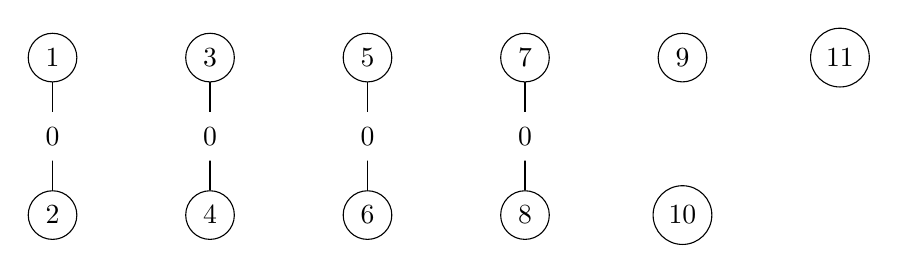
\begin{tikzpicture}

        \begin{scope}[every node/.style={circle,draw}]
          \node (1)  at (0,2)  {1};
          \node (2)  at (0,0)  {2};
          \node (3)  at (2,2)  {3};
          \node (4)  at (2,0)  {4};
          \node (5)  at (4,2)  {5};
          \node (6)  at (4,0)  {6};
          \node (7)  at (6,2)  {7};
          \node (8)  at (6,0)  {8};
          \node (9)  at (8,2)  {9};
          \node (10) at (8,0)  {10};
          \node (11) at (10,2) {11};
        \end{scope}

        \begin{scope}[every node/.style={fill=white,circle}]

          \begin{scope}[every edge/.style={draw}]
            \path (1)  edge node {$0$} (2);
            \path (3)  edge node {$0$} (4);
            \path (5)  edge node {$0$} (6);
            \path (7)  edge node {$0$} (8);
          \end{scope}
        \end{scope}

      \end{tikzpicture}
      \caption{$\rho_0$ est une 4-transposition}
    \end{center}
  \end{figure}

  \paragraph{}
  Now, let's form an alternation square between $\rho_0$ and $\rho_4$.

  \begin{figure}[H]
    \begin{center}
      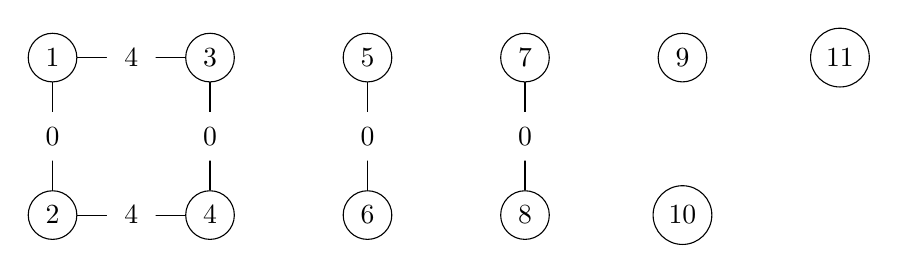
\begin{tikzpicture}

        \begin{scope}[every node/.style={circle,draw}]
          \node (1)  at (0,2)  {1};
          \node (2)  at (0,0)  {2};
          \node (3)  at (2,2)  {3};
          \node (4)  at (2,0)  {4};
          \node (5)  at (4,2)  {5};
          \node (6)  at (4,0)  {6};
          \node (7)  at (6,2)  {7};
          \node (8)  at (6,0)  {8};
          \node (9)  at (8,2)  {9};
          \node (10) at (8,0)  {10};
          \node (11) at (10,2) {11};
        \end{scope}

        \begin{scope}[every node/.style={fill=white,circle}]

          \begin{scope}[every edge/.style={draw}]
            \path (1)  edge node {$0$} (2);
            \path (3)  edge node {$0$} (4);
            \path (5)  edge node {$0$} (6);
            \path (7)  edge node {$0$} (8);
            \path (1)  edge node {$4$} (3);
            \path (2)  edge node {$4$} (4);
          \end{scope}
        \end{scope}

      \end{tikzpicture}
      \caption{Cas 1: carré alterné}
    \end{center}
  \end{figure}

  \paragraph{}
  By Lemma~\ref{lemma-continue-alternating-square}, we need to find one sequence of alternating squares until the difference between indices is two. Therefore this sequence contains at least 3 squares. It's impossible to have 5 squares because we only have 11 points. So the sequence is monotone and so linear.

  \paragraph{}
  From the square $[\rho_0, \rho_4]$, we can go to the square $[\rho_1, \rho_4]$ or to the square $[\rho_0, \rho_3]$. But we must use the edges of involution $\rho_0$ now, the two remaining $\rho_0$ edges use 4 points and the sequence of three squares uses 8 points thus they must share at least one point. But no $\rho_0$ edge can be connected to the sequence of alternating square because an $[\rho_{-1}, \rho_1]$ square will be needed to do this but $\rho_{-1}$ does not exist. We cannot use them later in the sequence of alternating square because it is monotone and so, it will never go back to $\rho_0$ once it leave it. The only solution is that the sequence of alternating square must used a $\rho_0$ edge in the next square. The following square in the sequence is therefore $[\rho_0, \rho_3]$.

  \paragraph{}
  Because the sequence is linear, the following square must be $[\rho_0, \rho_2]$. It's the third square and the difference between indices is only two, so we can stop here. For now we have the following graph:


  \begin{figure}[H]
    \begin{center}
      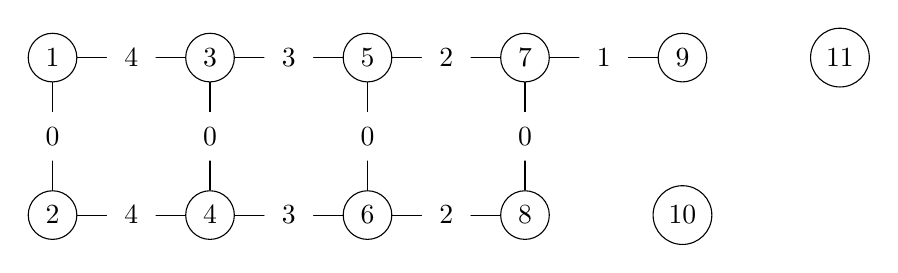
\begin{tikzpicture}

        \begin{scope}[every node/.style={circle,draw}]
          \node (1)  at (0,2)  {1};
          \node (2)  at (0,0)  {2};
          \node (3)  at (2,2)  {3};
          \node (4)  at (2,0)  {4};
          \node (5)  at (4,2)  {5};
          \node (6)  at (4,0)  {6};
          \node (7)  at (6,2)  {7};
          \node (8)  at (6,0)  {8};
          \node (9)  at (8,2)  {9};
          \node (10) at (8,0)  {10};
          \node (11) at (10,2) {11};
        \end{scope}

        \begin{scope}[every node/.style={fill=white,circle}]

          \begin{scope}[every edge/.style={draw}]
            \path (1)  edge node {$0$} (2);
            \path (3)  edge node {$0$} (4);
            \path (5)  edge node {$0$} (6);
            \path (7)  edge node {$0$} (8);
            \path (7)  edge node {$1$} (9);
            \path (5)  edge node {$2$} (7);
            \path (6)  edge node {$2$} (8);
            \path (3)  edge node {$3$} (5);
            \path (4)  edge node {$3$} (6);
            \path (1)  edge node {$4$} (3);
            \path (2)  edge node {$4$} (4);
          \end{scope}
        \end{scope}

      \end{tikzpicture}
      \caption{Cas 1.1: doubles carrés alternés}
    \end{center}
  \end{figure}

  \paragraph{}
  To link the two remaining points, we only need two edges but the total amount of edge will be odd but that is fordidden because we want that the generated group is $A_{11}$. To restore parity we need to create a double edge or an alternating square. The number of points if insufficient to create an alternating square, so we must create a double edge and the difference between its indices must be two. All $\rho_0$ edges have already be used, so the possibilities for double edges are $(\rho_1, \rho_3)$ and $(\rho_2, \rho_4)$ but then the number of $\rho_3$ or $\rho_4$ edge becomes odd. So it is impossible to connect all points if $\rho_0$ is a 4-transposition and there is an alternating square between $\rho_0$ and $\rho_4$.
\end{proof}

\begin{lemma}
  \label{lemma-forbidden-double-edge}
  In a permutation representation graph of rank 5 with 11 points, it's impossible to have a double edge between $\rho_0$ and $\rho_4$.
\end{lemma}

\begin{proof}
  By Lemme~\ref{lemma-extend-double-edge}
  To extend a double edge $(\rho_0, \rho_4)$, we must use an alternating square, we have two possibilities, either $[\rho_0, \rho_3]$ or $[\rho_1, \rho_4]$. Those two solutions are dual, so we will only study the first one. This square must then be extended to $[\rho_0, \rho_2]$ because we must stay linear. We have the following graph:

  \begin{figure}[H]
    \begin{center}
      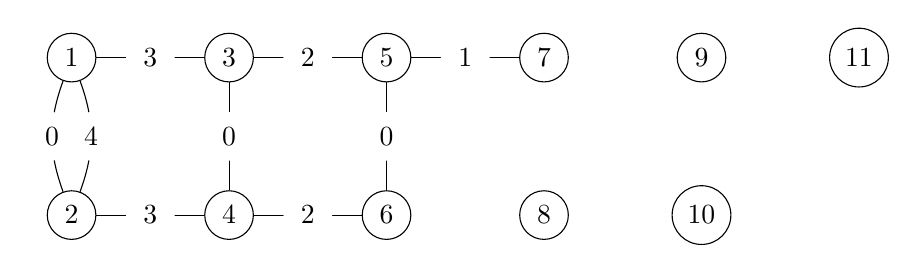
\begin{tikzpicture}

        \begin{scope}[every node/.style={circle,draw}]
          \node (1)  at (0,2)  {1};
          \node (2)  at (0,0)  {2};
          \node (3)  at (2,2)  {3};
          \node (4)  at (2,0)  {4};
          \node (5)  at (4,2)  {5};
          \node (6)  at (4,0)  {6};
          \node (7)  at (6,2)  {7};
          \node (8)  at (6,0)  {8};
          \node (9)  at (8,2)  {9};
          \node (10) at (8,0)  {10};
          \node (11) at (10,2) {11};
        \end{scope}

        \begin{scope}[every node/.style={fill=white,circle}]

          \begin{scope}[every edge/.style={draw}]
            \path (1)  edge[bend right=20] node {$0$} (2);
            \path (3)  edge node {$0$} (4);
            \path (5)  edge node {$0$} (6);
            \path (5)  edge node {$1$} (7);
            \path (3)  edge node {$2$} (5);
            \path (4)  edge node {$2$} (6);
            \path (1)  edge node {$3$} (3);
            \path (2)  edge node {$3$} (4);
            \path (1)  edge[bend left=20] node {$4$} (2);
          \end{scope}
        \end{scope}

      \end{tikzpicture}
      \caption{Cas 1.1.2: doubles carrés alternés et arêtes doublées}
    \end{center}
  \end{figure}

  \paragraph{}
  We have two issues in this graphs: there is only one $\rho_4$ edge and if we link all remaining points with single edge, the total number of edges will be odd.

  \paragraph{}
  The $\rho_4$ edge cannot be place on the existing graph. So it must be placed between two fixed points. Then we need to link this edge to the rest of the graph, and because we have only two points, remaining, it must be done using a $\rho_2$ and $\rho_3$ edge. For now, we have the following graph:


  \begin{figure}[H]
    \begin{center}
      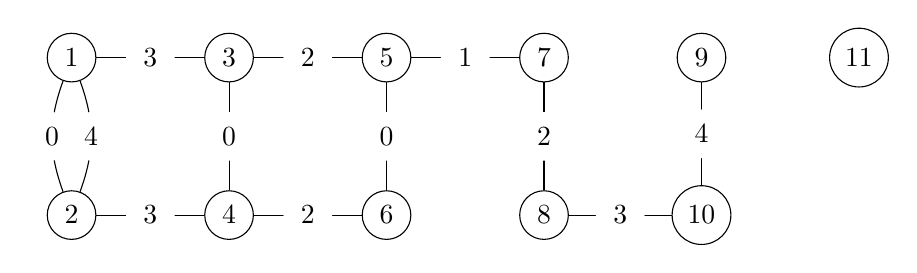
\begin{tikzpicture}

        \begin{scope}[every node/.style={circle,draw}]
          \node (1)  at (0,2)  {1};
          \node (2)  at (0,0)  {2};
          \node (3)  at (2,2)  {3};
          \node (4)  at (2,0)  {4};
          \node (5)  at (4,2)  {5};
          \node (6)  at (4,0)  {6};
          \node (7)  at (6,2)  {7};
          \node (8)  at (6,0)  {8};
          \node (9)  at (8,2)  {9};
          \node (10) at (8,0)  {10};
          \node (11) at (10,2) {11};
        \end{scope}

        \begin{scope}[every node/.style={fill=white,circle}]

          \begin{scope}[every edge/.style={draw}]
            \path (1)  edge[bend right=20] node {$0$} (2);
            \path (3)  edge node {$0$} (4);
            \path (5)  edge node {$0$} (6);
            \path (5)  edge node {$1$} (7);
            \path (3)  edge node {$2$} (5);
            \path (4)  edge node {$2$} (6);
            \path (7)  edge node {$2$} (8);
            \path (1)  edge node {$3$} (3);
            \path (2)  edge node {$3$} (4);
            \path (8)  edge node {$3$} (10);
            \path (1)  edge[bend left=20] node {$4$} (2);
            \path (9)  edge node {$4$} (10);
          \end{scope}
        \end{scope}

      \end{tikzpicture}
      \caption{Cas 1.1.2: doubles carrés alternés et arêtes doublées}
    \end{center}
  \end{figure}

  \paragraph{}
  If wa want that the total number of point must be even, we must link the last point we a double edge. But that is impossile because the only point where we can start a double edge is the end of the $\rho_4$ edge but the the double edge must be $(\rho_3, \rho_5)$ but $\rho_5$ does not exists. Thus we cannot have a double edge between $\rho_0$ and $\rho_4$ in a permutation representation graph of $A_{11}$.


\end{proof}

\subsection{Main theorems}

\begin{lemma}
  $\rho_0$ (and thus $\rho_4$) cannot be a 4-transposition.
\end{lemma}

\begin{proof}
  Takin the graph with only the $\rho_0$ 4-transposition, the $\rho_4$ involution must now be added but must commute with $\rho_0$. The following patterns are
  \begin{enumerate}
    \item Form an alternating square
    \item Double an existing edge
    \item Link two fixed points
  \end{enumerate}

  \paragraph{}
  The last pattern can only be user once because we only have three fixed points. But either $\rho_4$ is a 4-transposition or a 2-transposition, it is, at least, one edge to must still be placed. Thus, we must use one of the two other possibilities but we know that they do not lead to anything. So $\rho_4$ cannot be a 4-transposition.

\end{proof}

We can now split our analysis in two cases dependending of the disposition of 4-tranpositions:
\begin{enumerate}
  \item $\rho_1$ and $\rho_3$ are 4-transpositions
  \item $\rho_1$ is a 4-transposition but $\rho_3$ is not.
  \item $\rho_1$ and $\rho_3$ are 2-transposition. If $\rho_3$ is a 4-transposition but $\rho_1$ not, we can take the dual and reduce it to the second case.
\end{enumerate}

\paragraph{}
The objective is to prove the following theorem in the two first cases:
\begin{theorem}
  If $\rho_1$ is a 4-transposition, then a generator can be written as a product of other generators, and thus the generating set is not free, so the group is not a sggi.
\end{theorem}

\paragraph{}
If this theorem is proven, no string C-group can belong to the two first cases.

\subsubsection{$\rho_1$ and $\rho_3$ are 4-transpositions}

\paragraph{}
We must place

\subsubsection{$\rho_1$ is a 4-transposition but $\rho_3$ is not}

\paragraph{}
Recall that, by Lemmas~\ref{lemma-forbidden-alternating-square} and~\ref{lemma-forbidden-double-edge}, we know that the edges of involutions $\rho_0$ and $\rho_4$ cannot share a vertex.

\paragraph{}
Let's draw a graph on which we draw all edges of the 4-transposition $\rho_1$. This transposition must commute with $\rho_3$ and $\rho_4$. We want to place the edge for $\rho_4$. They must commute with thoses of $\rho_1$, so for the two first edges, we have three possibilities: we can build an alternating square, double two edges or double one edge an link two fixed points.

\paragraph{}
Let's consider the first case, the alternating square:

\paragraph{}
If $\rho_4$ forms an alternating square with $\rho_1$, it must be adjacent to an other alternating square between $\rho_1$ and $\rho_3$ ($\rho_2$ and $\rho_4$ is not possible because $\rho_4$ is a 2-transposition). Thoses squares must be linked to the rest of the graph by a $\rho_2$ edge. Thus edge is not part of any alternating square, therefore it must link the square with the remaining $\rho_1$ edge. For now, we have the following graph:

\begin{figure}[H]
  \begin{center}
    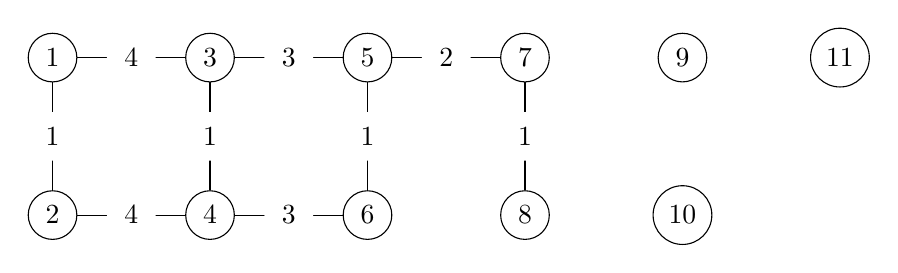
\begin{tikzpicture}

      \begin{scope}[every node/.style={circle,draw}]
        \node (1)  at (0,2)  {1};
        \node (2)  at (0,0)  {2};
        \node (3)  at (2,2)  {3};
        \node (4)  at (2,0)  {4};
        \node (5)  at (4,2)  {5};
        \node (6)  at (4,0)  {6};
        \node (7)  at (6,2)  {7};
        \node (8)  at (6,0)  {8};
        \node (9)  at (8,2)  {9};
        \node (10) at (8,0)  {10};
        \node (11) at (10,2) {11};
      \end{scope}

      \begin{scope}[every node/.style={fill=white,circle}]

        \begin{scope}[every edge/.style={draw}]
          \path (1)  edge node {$1$} (2);
          \path (3)  edge node {$1$} (4);
          \path (5)  edge node {$1$} (6);
          \path (7)  edge node {$1$} (8);
          \path (5)  edge node {$2$} (7);
          \path (3)  edge node {$3$} (5);
          \path (4)  edge node {$3$} (6);
          \path (1)  edge node {$4$} (3);
          \path (2)  edge node {$4$} (4);
        \end{scope}
      \end{scope}

    \end{tikzpicture}
    \caption{}
  \end{center}
\end{figure}

\paragraph{}
Now, if we try to place edges of $\rho_0$, we have a problem because we only have one available $\rho_1$ edge to link them to the rest. Therefore we need to from an alternating square between $\rho_0$ and $\rho_2$ and link it with the $\rho_1$ edge. We have the following graph:
% TODO une petite preuve ?

\begin{figure}[H]
  \begin{center}
    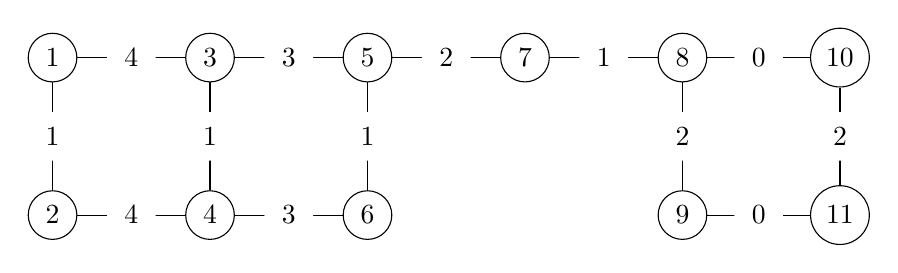
\begin{tikzpicture}

      \begin{scope}[every node/.style={circle,draw}]
        \node (1)  at (0,2)  {1};
        \node (2)  at (0,0)  {2};
        \node (3)  at (2,2)  {3};
        \node (4)  at (2,0)  {4};
        \node (5)  at (4,2)  {5};
        \node (6)  at (4,0)  {6};
        \node (7)  at (6,2)  {7};
        \node (8)  at (8,2)  {8};
        \node (9)  at (8,0)  {9};
        \node (10) at (10,2)  {10};
        \node (11) at (10,0) {11};
      \end{scope}

      \begin{scope}[every node/.style={fill=white,circle}]

        \begin{scope}[every edge/.style={draw}]
          \path (9)  edge node {$0$} (11);
          \path (8)  edge node {$0$} (10);
          \path (1)  edge node {$1$} (2);
          \path (3)  edge node {$1$} (4);
          \path (5)  edge node {$1$} (6);
          \path (7)  edge node {$1$} (8);
          \path (5)  edge node {$2$} (7);
          \path (8)  edge node {$2$} (9);
          \path (10) edge node {$2$} (11);
          \path (3)  edge node {$3$} (5);
          \path (4)  edge node {$3$} (6);
          \path (1)  edge node {$4$} (3);
          \path (2)  edge node {$4$} (4);
        \end{scope}
      \end{scope}

    \end{tikzpicture}
    \caption{Un carré alterné et son voisin engendré}
  \end{center}
\end{figure}

\paragraph{}
To restore parity, we still need to place a $\rho_2$ edge. There is only one posibility for a such edge: we need to double a $\rho_4$ edge, there are two of them.

\paragraph{}
Now we can stop here and $\rho_3$ will be a 2-transposition or we can add two extra $\rho_3$ edges. Those edges must be located between points $1$ and $2$, and between points $10$ et $11$.

\paragraph{}
If $\rho_3$ is a 4-transposition then the graph is the following:

\begin{figure}[H]
  \begin{center}
    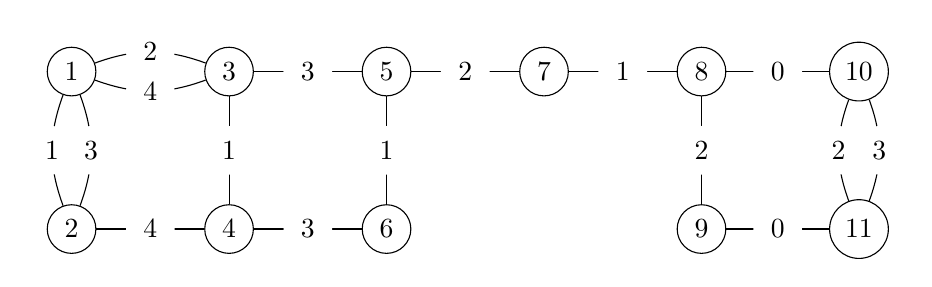
\begin{tikzpicture}

      \begin{scope}[every node/.style={circle,draw}]
        \node (1)  at (0,2)  {1};
        \node (2)  at (0,0)  {2};
        \node (3)  at (2,2)  {3};
        \node (4)  at (2,0)  {4};
        \node (5)  at (4,2)  {5};
        \node (6)  at (4,0)  {6};
        \node (7)  at (6,2)  {7};
        \node (8)  at (8,2)  {8};
        \node (9)  at (8,0)  {9};
        \node (10) at (10,2)  {10};
        \node (11) at (10,0) {11};
      \end{scope}

      \begin{scope}[every node/.style={fill=white,circle}]

        \begin{scope}[every edge/.style={draw}]
          \path (9)  edge node {$0$} (11);
          \path (8)  edge node {$0$} (10);
          \path (1)  edge[bend right=20] node {$1$} (2);
          \path (3)  edge node {$1$} (4);
          \path (5)  edge node {$1$} (6);
          \path (7)  edge node {$1$} (8);
          \path (1)  edge[bend left=20] node {$2$} (3);
          \path (5)  edge node {$2$} (7);
          \path (8)  edge node {$2$} (9);
          \path (10) edge[bend right=20] node {$2$} (11);
          \path (1)  edge[bend left=20] node {$3$} (2);
          \path (3)  edge node {$3$} (5);
          \path (4)  edge node {$3$} (6);
          \path (10) edge[bend left=20] node {$3$} (11);
          \path (1)  edge[bend right=20] node {$4$} (3);
          \path (2)  edge node {$4$} (4);
        \end{scope}
      \end{scope}

    \end{tikzpicture}
    \caption{Un carré alterné et son voisin engendré}
  \end{center}
\end{figure}

\paragraph{}
Let's remove all edges from involutions $\rho_0$ and $\rho_3$, We have the following graph.

\begin{figure}[H]
  \begin{center}
    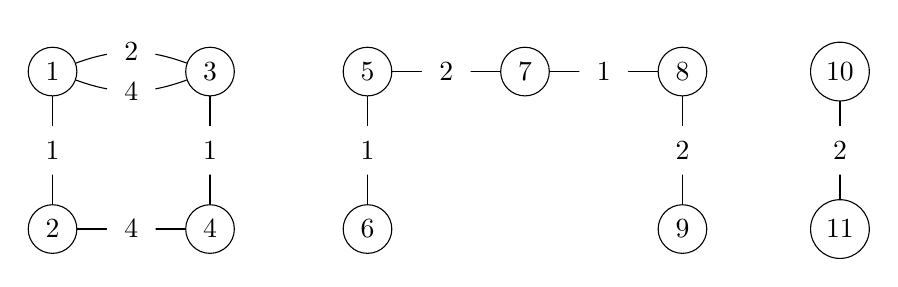
\begin{tikzpicture}

      \begin{scope}[every node/.style={circle,draw}]
        \node (1)  at (0,2)  {1};
        \node (2)  at (0,0)  {2};
        \node (3)  at (2,2)  {3};
        \node (4)  at (2,0)  {4};
        \node (5)  at (4,2)  {5};
        \node (6)  at (4,0)  {6};
        \node (7)  at (6,2)  {7};
        \node (8)  at (8,2)  {8};
        \node (9)  at (8,0)  {9};
        \node (10) at (10,2)  {10};
        \node (11) at (10,0) {11};
      \end{scope}

      \begin{scope}[every node/.style={fill=white,circle}]

        \begin{scope}[every edge/.style={draw}]
          \path (1)  edge node {$1$} (2);
          \path (3)  edge node {$1$} (4);
          \path (5)  edge node {$1$} (6);
          \path (7)  edge node {$1$} (8);
          \path (1)  edge[bend left=20] node {$2$} (3);
          \path (5)  edge node {$2$} (7);
          \path (8)  edge node {$2$} (9);
          \path (10) edge node {$2$} (11);
          \path (1)  edge[bend right=20] node {$4$} (3);
          \path (2)  edge node {$4$} (4);
        \end{scope}
      \end{scope}

    \end{tikzpicture}
    \caption{Un carré alterné et son voisin engendré}
  \end{center}
\end{figure}

\paragraph{}
Now we can see easily that $\rho_4 = (\rho_1 \rho_2)^{10}$. The set of generators is not free and so it's not a generating set.

\paragraph{}
This conclude our analysis for the alternating square between $\rho_1$ and $\rho_4$. The second possibility is having a double edge with involutions $\rho_0$ and $\rho_4$. We must place an alternating square next to it because this double must be connected to the rest of the graph. We have two possibilities for the alternating square: $[\rho_1, \rho_3]$ or $[\rho_2, \rho_4]$. In the first case, we have the following graph:

\begin{figure}[H]
  \begin{center}
    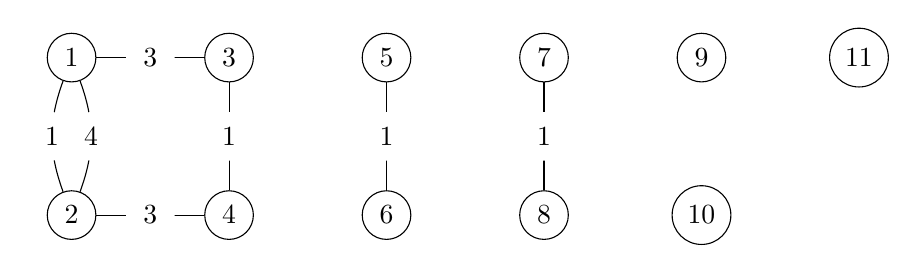
\begin{tikzpicture}

      \begin{scope}[every node/.style={circle,draw}]
        \node (1)  at (0,2)  {1};
        \node (2)  at (0,0)  {2};
        \node (3)  at (2,2)  {3};
        \node (4)  at (2,0)  {4};
        \node (5)  at (4,2)  {5};
        \node (6)  at (4,0)  {6};
        \node (7)  at (6,2)  {7};
        \node (8)  at (6,0)  {8};
        \node (9)  at (8,2)  {9};
        \node (10) at (8,0)  {10};
        \node (11) at (10,2) {11};
      \end{scope}

      \begin{scope}[every node/.style={fill=white,circle}]

        \begin{scope}[every edge/.style={draw}]
          \path (1)  edge[bend right=20] node {$1$} (2);
          \path (3)  edge node {$1$} (4);
          \path (5)  edge node {$1$} (6);
          \path (7)  edge node {$1$} (8);
          \path (1)  edge node {$3$} (3);
          \path (2)  edge node {$3$} (4);
          \path (1)  edge[bend left=20] node {$4$} (2);
        \end{scope}
      \end{scope}

    \end{tikzpicture}
    \caption{Un carré alterné et son voisin engendré}
  \end{center}
\end{figure}

\paragraph{}
In the second case, it's simpler and we have the following graph:


\begin{figure}[H]
  \begin{center}
    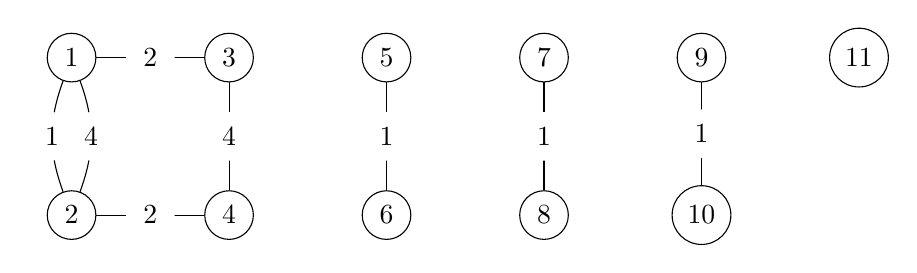
\begin{tikzpicture}

      \begin{scope}[every node/.style={circle,draw}]
        \node (1)  at (0,2)  {1};
        \node (2)  at (0,0)  {2};
        \node (3)  at (2,2)  {3};
        \node (4)  at (2,0)  {4};
        \node (5)  at (4,2)  {5};
        \node (6)  at (4,0)  {6};
        \node (7)  at (6,2)  {7};
        \node (8)  at (6,0)  {8};
        \node (9)  at (8,2)  {9};
        \node (10) at (8,0)  {10};
        \node (11) at (10,2) {11};
      \end{scope}

      \begin{scope}[every node/.style={fill=white,circle}]

        \begin{scope}[every edge/.style={draw}]
          \path (1)  edge[bend right=20] node {$1$} (2);
          \path (5)  edge node {$1$} (6);
          \path (7)  edge node {$1$} (8);
          \path (9)  edge node {$1$} (10);
          \path (1)  edge node {$2$} (3);
          \path (2)  edge node {$2$} (4);
          \path (1)  edge[bend left=20] node {$4$} (2);
          \path (3)  edge node {$4$} (4);
        \end{scope}
      \end{scope}

    \end{tikzpicture}
    \caption{Un carré alterné et son voisin engendré}
  \end{center}
\end{figure}

\paragraph{}
Now if we want to connect the alternating square to the rest of the graph, we must use a $\rho_3$ edge. But we cannot connect to a $\rho_1$ edge because we will need to build an alterating square and we will double the edge (and so it can be reduced to the previous case).

\paragraph{}
Now, this edge must be linked to the fixed point. And we need another edge that goes from the fixed point to a $\rho_1$ edge. We must use a $\rho_2$ edge. We cannot make an alternating square because in this case, a $\rho_1$ edge should leave the point that we just used. But it was fixed before we use it and so no $\rho_1$ touch it.

\paragraph{}
Let's notice that, for now, we need to place at least two double edges or alternating square if we want to complete the graph. It it the followin for now.

\begin{figure}[H]
  \begin{center}
    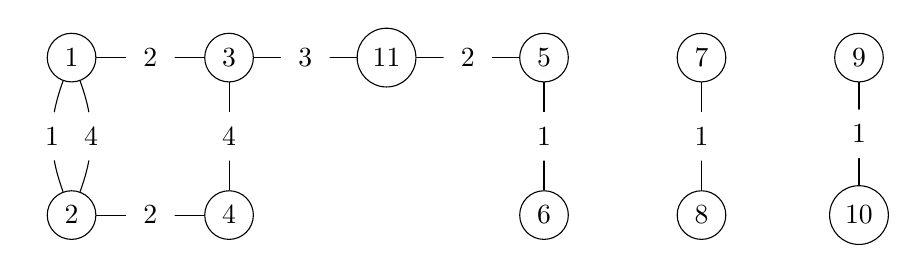
\begin{tikzpicture}

      \begin{scope}[every node/.style={circle,draw}]
        \node (1)  at (0,2)  {1};
        \node (2)  at (0,0)  {2};
        \node (3)  at (2,2)  {3};
        \node (4)  at (2,0)  {4};
        \node (11) at (4,2) {11};
        \node (5)  at (6,2)  {5};
        \node (6)  at (6,0)  {6};
        \node (7)  at (8,2)  {7};
        \node (8)  at (8,0)  {8};
        \node (9)  at (10,2) {9};
        \node (10) at (10,0) {10};
      \end{scope}

      \begin{scope}[every node/.style={fill=white,circle}]

        \begin{scope}[every edge/.style={draw}]
          \path (1)  edge[bend right=20] node {$1$} (2);
          \path (5)  edge node {$1$} (6);
          \path (7)  edge node {$1$} (8);
          \path (9)  edge node {$1$} (10);
          \path (1)  edge node {$2$} (3);
          \path (2)  edge node {$2$} (4);
          \path (5)  edge node {$2$} (11);
          \path (3)  edge node {$3$} (11);
          \path (1)  edge[bend left=20] node {$4$} (2);
          \path (3)  edge node {$4$} (4);
        \end{scope}
      \end{scope}

    \end{tikzpicture}
    \caption{Un carré alterné et son voisin engendré}
  \end{center}
\end{figure}



\begin{theorem}
  Let be a sggi of rank 5 on $A_{11}$. Then this sggi contains exactly a 4-transposition.
\end{theorem}

\paragraph{}
We must analyse two cases: the one who has two 4-tranpsositions (they will necessaraly be $\rho_1$ and $\rho_2$) and the one who has three 4-transpositions (in $\rho_1$, $\rho_2$ and $\rho_3$).

\begin{proof}
  Let's start with the graph of the previous proof, if we add the involutions $\rho_3$
  En partant du graphe de la preuve précédente, si on rajoute l'involution $\rho_3$, on l'étend à $A_{11}$.
  En effet, partons du graphe et essayons de rajouter la 2-transposition $\rho_3$, celle-ci doit commuter avec $\rho_0$ et $\rho_1$.
  \begin{figure}[H]
    \begin{center}
      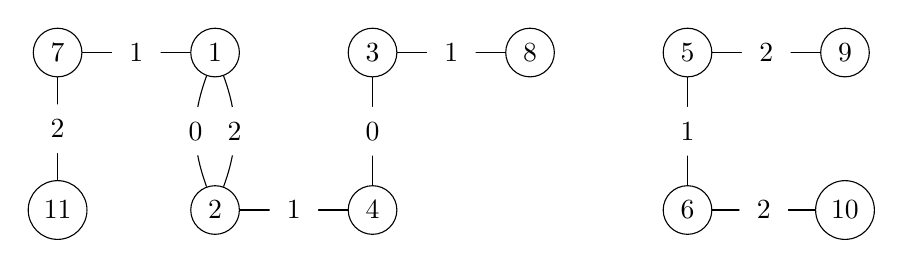
\begin{tikzpicture}

        \begin{scope}[every node/.style={circle,draw}]
          \node (1)  at (0,2)  {1};
          \node (2)  at (0,0)  {2};
          \node (3)  at (2,2)  {3};
          \node (4)  at (2,0)  {4};
          \node (5)  at (6,2)  {5};
          \node (6)  at (6,0)  {6};
          \node (7)  at (-2,2) {7};
          \node (8)  at (4,2)  {8};
          \node (9)  at (8,2)  {9};
          \node (10) at (8,0) {10};
          \node (11) at (-2,0) {11};
        \end{scope}

        \begin{scope}[every node/.style={fill=white,circle}]

          \begin{scope}[every edge/.style={draw}]
            \path (1)  edge[bend right=20] node {$0$} (2);
            \path (3)  edge node {$0$} (4);
            \path (1)  edge node {$1$} (7);
            \path (2)  edge node {$1$} (4);
            \path (3)  edge node {$1$} (8);
            \path (5)  edge node {$1$} (6);
            \path (1)  edge[bend left=20] node {$2$} (2);
            \path (5)  edge node {$2$} (9);
            \path (6)  edge node {$2$} (10);
            \path (7)  edge node {$2$} (11);
          \end{scope}
        \end{scope}

      \end{tikzpicture}
      \caption{Example of subgroup of sggi of type 2}
    \end{center}
  \end{figure}

  \paragraph{}
  Nous devons utiliser 2 arêtes $\rho_3$, pour cela nous avons trois possibilités, sachant que nous pouvons ignorer les arêtes $\rho_2$.
  \begin{enumerate}
    \item Relier deux points non reliés
    \item Doubler une arête
    \item Former un carré alterné
  \end{enumerate}

  \paragraph{}
  Dans la composante de gauche, suite à l'alternance des arêtes $\rho_0$ et $\rho_1$ il n'est pas possible de former un carré alterné ou une arête double, la seule possibilité est une arête qui partirait du point 11. Dans la composante de droite, les possibilités sont plus variés. On doit placer deux arêtes en tout et pour le moment nous n'avons trouvé qu'un point d'attache potentiel. Il en faut donc au moins 3 autres parmi les 4 points qui compose cette composante. Nous sommes donc obligé d'utiliser le point 5 ou le point 6 mais dans ce cas, nous sommes obligés de doubler l'arête $\rho_1$ présente à cet endroit. Pour la dernière arête soit nous relions les deux points restants dans la composante de droite soit nous relions un de ces points à l'autre composante.

  \paragraph{}
  Dans le premier cas nous ne pourrons jamais atteindre $A_{11}$. En effet, nous avons le graphe suivant
  \begin{figure}[H]
    \begin{center}
      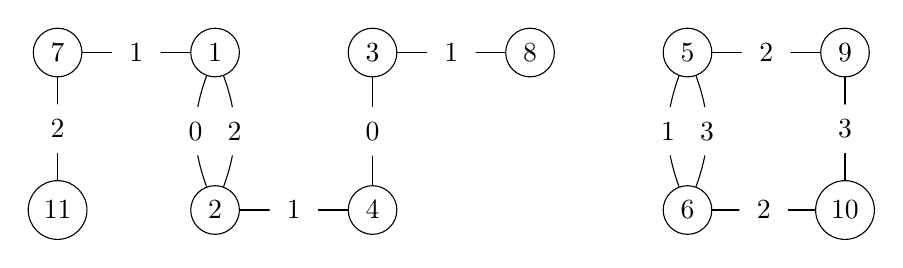
\begin{tikzpicture}

        \begin{scope}[every node/.style={circle,draw}]
          \node (1)  at (0,2)  {1};
          \node (2)  at (0,0)  {2};
          \node (3)  at (2,2)  {3};
          \node (4)  at (2,0)  {4};
          \node (5)  at (6,2)  {5};
          \node (6)  at (6,0)  {6};
          \node (7)  at (-2,2) {7};
          \node (8)  at (4,2)  {8};
          \node (9)  at (8,2)  {9};
          \node (10) at (8,0) {10};
          \node (11) at (-2,0) {11};
        \end{scope}

        \begin{scope}[every node/.style={fill=white,circle}]

          \begin{scope}[every edge/.style={draw}]
            \path (1)  edge[bend right=20] node {$0$} (2);
            \path (3)  edge node {$0$} (4);
            \path (1)  edge node {$1$} (7);
            \path (2)  edge node {$1$} (4);
            \path (3)  edge node {$1$} (8);
            \path (5)  edge[bend right=20] node {$1$} (6);
            \path (1)  edge[bend left=20] node {$2$} (2);
            \path (5)  edge node {$2$} (9);
            \path (6)  edge node {$2$} (10);
            \path (7)  edge node {$2$} (11);
            \path (5)  edge[bend left=20] node {$3$} (6);
            \path (9)  edge node {$3$} (10);
          \end{scope}
        \end{scope}

      \end{tikzpicture}
      \caption{Example of subgroup of sggi of type 2}
    \end{center}
  \end{figure}

  \paragraph{}
  Dans cet graphe, $\rho_2$ et $\rho_3$ commute donc ce graphe ne peut être celui d'un groupe semi-simple. Même si nous rajoutons des involutions, cela ne changera rien à ce résultat et le graphe ne pourra jamais être celui d'$A_{11}$. La seule possibilité qu'il nous reste est le premier graphe.

  \begin{figure}[H]
    \begin{center}
      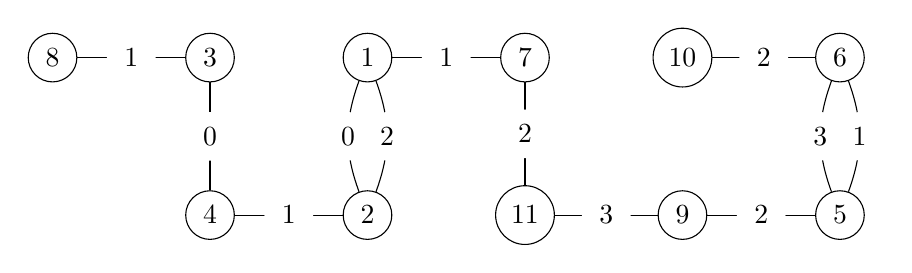
\begin{tikzpicture}

        \begin{scope}[every node/.style={circle,draw}]
          \node (1)  at (2,2)  {1};
          \node (2)  at (2,0)  {2};
          \node (3)  at (0,2)  {3};
          \node (4)  at (0,0)  {4};
          \node (5)  at (8,0)  {5};
          \node (6)  at (8,2)  {6};
          \node (7)  at (4,2)  {7};
          \node (8)  at (-2,2) {8};
          \node (9)  at (6,0)  {9};
          \node (10) at (6,2) {10};
          \node (11) at (4,0) {11};
        \end{scope}

        \begin{scope}[every node/.style={fill=white,circle}]

          \begin{scope}[every edge/.style={draw}]
            \path (1)  edge[bend right=20] node {$0$} (2);
            \path (3)  edge node {$0$} (4);
            \path (1)  edge node {$1$} (7);
            \path (2)  edge node {$1$} (4);
            \path (3)  edge node {$1$} (8);
            \path (5)  edge[bend right=20] node {$1$} (6);
            \path (1)  edge[bend left=20] node {$2$} (2);
            \path (5)  edge node {$2$} (9);
            \path (6)  edge node {$2$} (10);
            \path (7)  edge node {$2$} (11);
            \path (5)  edge[bend left=20] node {$3$} (6);
            \path (9)  edge node {$3$} (11);
          \end{scope}
        \end{scope}

      \end{tikzpicture}
      \caption{Example of subgroup of sggi of type 2}
    \end{center}
  \end{figure}

\end{proof}

\begin{lemma}
  Ce graphe engendre $A_{11}$.
\end{lemma}

\subsubsection{$\rho_1$ n'est pas une 4-transposition}

\paragraph{}
Par le lemme précédent, il faut au moins une 4-transposition. Celle-ci doit forcément se trouver en $\rho_2$.

\paragraph{}
Dans ce cas, aucun générateur n'est redondante. En effet si on supprimait un générateur, on aurait un sggi de rang 4 avec une seule 4-transposition mais nous avons prouvé que, dans ce cas, il ne peut engendrer $A_11$.

\paragraph{}
Commençons par trouver tous les sggis de rang 5 qui sont valables.

\begin{theorem}
  Les seuls graphes CPR de rang 5 sur 11 points sont ceux présents à la section~\ref{monodromy-5} (p.~\pageref{monodromy-5}).

\end{theorem}

\paragraph{}
Nous devons prouver qu'il n'y a aucun C-group de rang 5 qui engendre $A_{11}$.

\begin{theorem}
  Soit un sggi de rang 5 sur $A_{11}$. Alors ce sggi n'est pas un C-group.
\end{theorem}

\begin{proof}
  Nous allons construire toutes les possibilités de graphe CPR. Partons d'un graphe avec juste la 4-transposition $\rho_2$.

  \begin{figure}[H]
    \begin{center}
      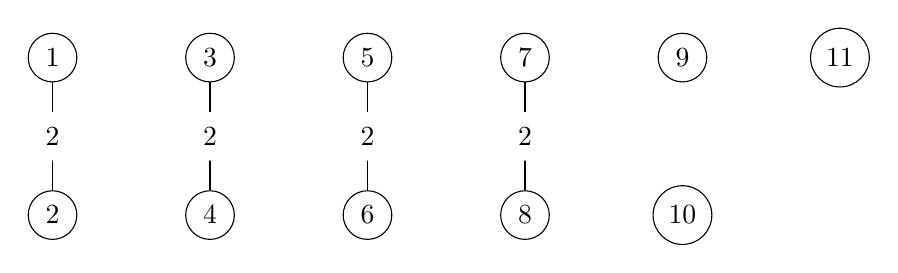
\begin{tikzpicture}

        \begin{scope}[every node/.style={circle,draw}]
          \node (1)  at (0,2)  {1};
          \node (2)  at (0,0)  {2};
          \node (3)  at (2,2)  {3};
          \node (4)  at (2,0)  {4};
          \node (5)  at (4,2)  {5};
          \node (6)  at (4,0)  {6};
          \node (7)  at (6,2)  {7};
          \node (8)  at (6,0)  {8};
          \node (9)  at (8,2)  {9};
          \node (10) at (8,0)  {10};
          \node (11) at (10,2) {11};
        \end{scope}

        \begin{scope}[every node/.style={fill=white,circle}]

          \begin{scope}[every edge/.style={draw}]
            \path (1)  edge node {$2$} (2);
            \path (3)  edge node {$2$} (4);
            \path (5)  edge node {$2$} (6);
            \path (7)  edge node {$2$} (8);
          \end{scope}
        \end{scope}

      \end{tikzpicture}
      \caption{[1, 5, 1010, 232, 381]}
    \end{center}
  \end{figure}

\paragraph{}
Nous allons essayer d'ajouter les involutions $\rho_0$ et $\rho_4$. Celles-ci doivent commuter avec $\rho_2$. Pour chaque involution nous devons choisir entre les 3 possibilités suivantes:
\begin{enumerate}
  \item Faire un arête double avec $\rho_2$ et reliés deux points qui sont, pour le moment, fixes.
  \item Faire deux arêtes doubles avec $\rho_2$.
  \item Faire un carré alterné avec $\rho_2$.
\end{enumerate}

\paragraph{}
S'il n'y a qu'une seule 4-transposition, alors nous avons 12 arêtes pour relier 11 points soit 2 de plus que le strict minimum. Dès lors, lorsque nous ajoutons une arête, elle doit toujours relier deux composantes différentes, sauf à deux occasions. Quand nous formons un carré alterné, nous utilisons une de ces deux arêtes et il se passe la même chose quand nous formons une arête double.

\paragraph{}
Parmi les trois possibilités, la seconde est impossible car si nous l'appliquons, nous aurons déjà utilisé nous deux arêtes "joker". Quand nous allons vouloir ajouter la seconde involution, nous n'en aurons plus mais toutes les possibilités en demande au moins une.

\paragraph{}
Remarquons qu'il est impossible de faire le même choix pour $\rho_0$ et $\rho_4$. Si nous utilisions deux fois la première proposition, il nous faudrait 4 points fixes mais nous n'en avons que 3. Si nous choisissons la troisième proposition, nous ne pouvons pas superposer les carrés sans former deux arêtes doubles, ce qui est impossible.

\paragraph{}
Les deux carrés ne peuvent pas être adjacents non plus car on aurait des arêtes $\rho_0$ et $\rho_4$ adjacentes mais nous ne pourions plus former de carré alterné pour créer un motif valable.

\paragraph{}
Dans le cas deux deux carrés disjoints, nous ne pouvons pas les relier car nous avons utilisé toutes les arêtes des involutions $\rho_0$, $\rho_2$ et $\rho_4$. Il ne nous reste donc que des arêtes des involutions $\rho_1$ et $\rho_3$ et celles-ce ne peuvent partager un sommet sans former un carré alterné ou une arêted double mais ça c'est impossible.

\paragraph{}
La seule possibilité qu'il nous reste est de choisir que $\rho_0$ reliera deux point fixes et doublera une arête et que $\rho_4$ formera un carré alterné (l'autre cas est le dual). On a donc le graphe suivant:


\begin{figure}[H]
  \begin{center}
    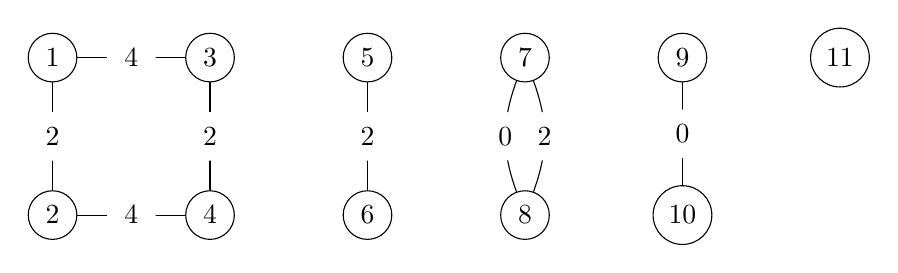
\begin{tikzpicture}

      \begin{scope}[every node/.style={circle,draw}]
        \node (1)  at (0,2)  {1};
        \node (2)  at (0,0)  {2};
        \node (3)  at (2,2)  {3};
        \node (4)  at (2,0)  {4};
        \node (5)  at (4,2)  {5};
        \node (6)  at (4,0)  {6};
        \node (7)  at (6,2)  {7};
        \node (8)  at (6,0)  {8};
        \node (9)  at (8,2)  {9};
        \node (10) at (8,0)  {10};
        \node (11) at (10,2) {11};
      \end{scope}

      \begin{scope}[every node/.style={fill=white,circle}]

        \begin{scope}[every edge/.style={draw}]
          \path (9)  edge node {$0$} (10);
          \path (7)  edge[bend right=20] node {$0$} (8);
          \path (1)  edge node {$2$} (2);
          \path (3)  edge node {$2$} (4);
          \path (5)  edge node {$2$} (6);
          \path (7)  edge[bend left=20] node {$2$} (8);
          \path (1)  edge node {$4$} (3);
          \path (2)  edge node {$4$} (4);
        \end{scope}
      \end{scope}

    \end{tikzpicture}
    \caption{[1, 5, 1010, 232, 381]}
  \end{center}
\end{figure}

\paragraph{}
À partir de maintenant, si nous rajoutons une arête, elle doit relier deux composantes connexes distinctes du graphe.

\paragraph{}
Le carré alterné doit être relié par une arête $\rho_3$. Cette arête peut aller sur le point fixe ou sur l'arête isolée $\rho_2$. Néanmoins du point fixe, il est impossible de continuer car il nous faut une arête $\rho_2$ ou $\rho_4$ mais elles ont toutes déjà été placées. Donc il y a une arête $\rho_3$ entre le carré alterné et l'arête isolée $\rho_2$.

\paragraph{}
Vu que nous n'avons qu'une arête $\rho_2$ isolée, nous n'avons qu'un moyen de relier les arêtes $\rho_1$ au carré. Toutes ces arêtes doivent donc être dans la même partie du graphe.

\paragraph{}
Remarquons que l'arête double $(\rho_0, \rho_2)$ ainsi que l'arête simple $\rho_0$ ne peuvent être relié que par des arête $\rho_1$. Vu que nous n'avons que deux arêtes $\rho_1$ et que toutes ces arêtes sont situés dans la même branche du graphe, une de ces arêtes doit être à l'extémité de la branche et doit être relié à l'autre avec une arête $\rho_1$. On stade actuel, nous avons le graphe suivant:

\begin{figure}[H]
  \begin{center}
    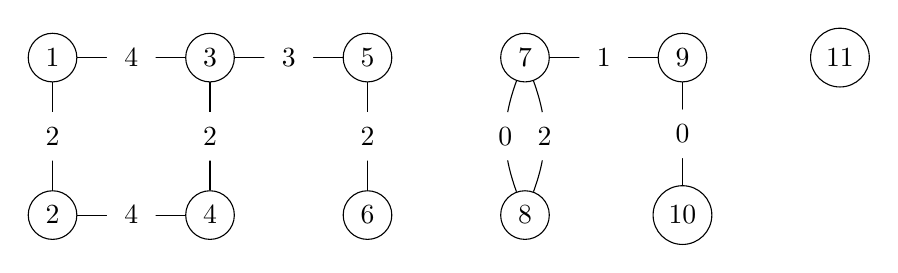
\begin{tikzpicture}

      \begin{scope}[every node/.style={circle,draw}]
        \node (1)  at (0,2)  {1};
        \node (2)  at (0,0)  {2};
        \node (3)  at (2,2)  {3};
        \node (4)  at (2,0)  {4};
        \node (5)  at (4,2)  {5};
        \node (6)  at (4,0)  {6};
        \node (7)  at (6,2)  {7};
        \node (8)  at (6,0)  {8};
        \node (9)  at (8,2)  {9};
        \node (10) at (8,0)  {10};
        \node (11) at (10,2) {11};
      \end{scope}

      \begin{scope}[every node/.style={fill=white,circle}]

        \begin{scope}[every edge/.style={draw}]
          \path (9)  edge node {$0$} (10);
          \path (7)  edge[bend right=20] node {$0$} (8);
          \path (7)  edge node {$1$} (9);
          \path (1)  edge node {$2$} (2);
          \path (3)  edge node {$2$} (4);
          \path (5)  edge node {$2$} (6);
          \path (7)  edge[bend left=20] node {$2$} (8);
          \path (3)  edge node {$3$} (5);
          \path (1)  edge node {$4$} (3);
          \path (2)  edge node {$4$} (4);
        \end{scope}
      \end{scope}

    \end{tikzpicture}
    \caption{[1, 5, 1010, 232, 381]}
  \end{center}
\end{figure}

\paragraph{}
À ce stade, il reste une arête $\rho_1$ et une arête $\rho_3$ à placer. L'arête $\rho_1$ permet de relier le l'arête simple $\rho_2$ à la grande composante. On a deux façons de le faire en fonction du sens dans lequel on attache cette dernière. L'arête $\rho_3$ quant à elle doit servir à relier le point fixe au reste. Le seul point d'attche pour cette arête $\rho_3$ est le carré alterné. On a trois possibilités, on fonction si les arêtes $\rho_3$ sont connectées à des sommets opposés sur le carré, si elles sont séparées par une arête $\rho_2$ ou une arête $\rho_4$.

\paragraph{}
En tout, on a donc exactement 6 graphe CPR admissibles pour cette configuration.

\end{proof}

From now, we are numeroting points of the graph in the same way as in section~\ref{monodromy-5} (p. \pageref{monodromy-5})

\begin{theorem}
  None of the groups generated by sggis reprensented on those graphs are C-group.
\end{theorem}

\begin{proof}
  By the definition of a C-group, it is sufficient to find two subsets of generators $S_1$ and $S_2$ such that $\Gamma_{S_1} \cap \Gamma_{S_2} \neq \Gamma_{S_1 \cap S_2}$.

  \paragraph{}
  In our case, let's take $S_1 = \{\rho_1, \rho_2\}$ and $S_2 = \{\rho_2, \rho_3, \rho_4\}$. Here $S_1 \cap S_2 = \{\rho_2\}$ and so $\Gamma_{\rho_2} = \langle (1\ 2)(5\ 6)(7\ 8)(9\ 10) \rangle$. This group is a cylic groupe of order 2, so it contains only two elements, identity and $\rho_2$. Hence, $\rho_2$ is an involution.

  \paragraph{}
  Let's study $S_1$ more deeply, if we only consider those generators the choice made while positioning $\rho_3$ in the alternating square does not have any importance. We have only two different graphs to study (it may be necessary to renumber some vertex):

  \begin{figure}[H]
    \begin{center}
      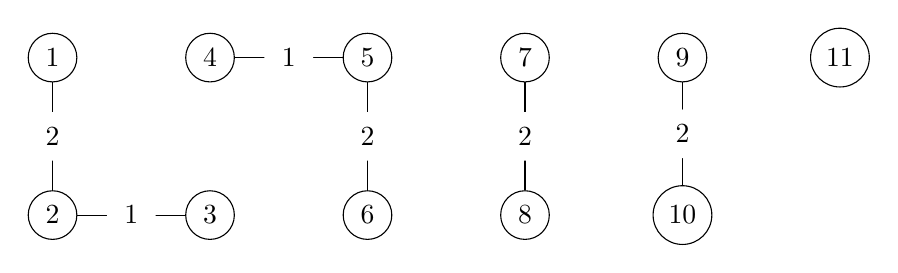
\begin{tikzpicture}

        \begin{scope}[every node/.style={circle,draw}]
          \node (1)  at (0,2)  {1};
          \node (2)  at (0,0)  {2};
          \node (3)  at (2,0)  {3};
          \node (4)  at (2,2)  {4};
          \node (5)  at (4,2)  {5};
          \node (6)  at (4,0)  {6};
          \node (7)  at (6,2)  {7};
          \node (8)  at (6,0)  {8};
          \node (9)  at (8,2)  {9};
          \node (10) at (8,0)  {10};
          \node (11) at (10,2) {11};
        \end{scope}

        \begin{scope}[every node/.style={fill=white,circle}]

          \begin{scope}[every edge/.style={draw}]
            \path (2)  edge node {$1$} (3);
            \path (4)  edge node {$1$} (5);
            \path (1)  edge node {$2$} (2);
            \path (5)  edge node {$2$} (6);
            \path (7)  edge node {$2$} (8);
            \path (9)  edge node {$2$} (10);
          \end{scope}
        \end{scope}

      \end{tikzpicture}
      \caption{[1, 5, 994, 219, 381]}
    \end{center}
  \end{figure}

  \begin{figure}[H]
    \begin{center}
      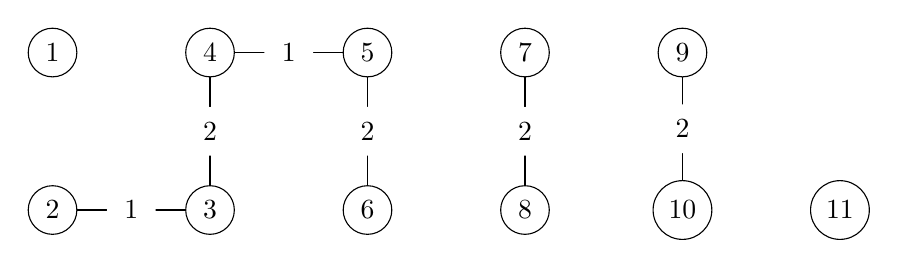
\begin{tikzpicture}

        \begin{scope}[every node/.style={circle,draw}]
          \node (1)  at (0,2)  {1};
          \node (2)  at (0,0)  {2};
          \node (3)  at (2,0)  {3};
          \node (4)  at (2,2)  {4};
          \node (5)  at (4,2)  {5};
          \node (6)  at (4,0)  {6};
          \node (7)  at (6,2)  {7};
          \node (8)  at (6,0)  {8};
          \node (9)  at (8,2)  {9};
          \node (10) at (8,0)  {10};
          \node (11) at (10,0) {11};
        \end{scope}

        \begin{scope}[every node/.style={fill=white,circle}]

          \begin{scope}[every edge/.style={draw}]
            \path (2)  edge node {$1$} (3);
            \path (4)  edge node {$1$} (5);
            \path (3)  edge node {$2$} (4);
            \path (5)  edge node {$2$} (6);
            \path (7)  edge node {$2$} (8);
            \path (9)  edge node {$2$} (10);
          \end{scope}
        \end{scope}

      \end{tikzpicture}
      \caption{[1, 5, 1010, 232, 381]}
    \end{center}
  \end{figure}

  \paragraph{}
  In the first graph, the permutation $(\rho_1 \rho_2)^2 \rho_1$, it lets points of the two isolated edge as-is because the permutation use $\rho_2$ an even number of times. Points 3 and 4 also remain in the same position. But points 1 and 2 as well as 5 and 6 are swaped. We have $(\rho_1 \rho_2)^2 \rho_1 = (1\ 2)(5\ 6) \in \Gamma_{S_1}$.

  \paragraph{}
  In the second graph, it's $(\rho_1\rho_2)^4 \rho_1$ that give us the same result.

  % TODO Renuméroter les graphes !!!

  \paragraph{}
  Now, let's study $S_2$, the way we have connected the tail to the alternating graph does not matter here. But the disposition of the edges alongside the alternating square is very important.

  \begin{figure}[H]
    \begin{center}
      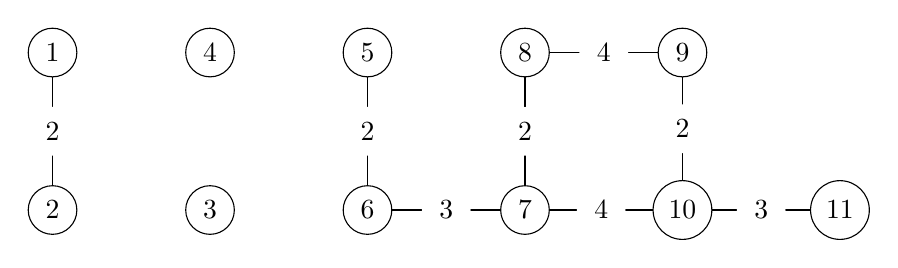
\begin{tikzpicture}

        \begin{scope}[every node/.style={circle,draw}]
          \node (1)  at (0,2)  {1};
          \node (2)  at (0,0)  {2};
          \node (3)  at (2,0)  {3};
          \node (4)  at (2,2)  {4};
          \node (5)  at (4,2)  {5};
          \node (6)  at (4,0)  {6};
          \node (7)  at (6,0)  {7};
          \node (8)  at (6,2)  {8};
          \node (9)  at (8,2)  {9};
          \node (10) at (8,0)  {10};
          \node (11) at (10,0) {11};
        \end{scope}

        \begin{scope}[every node/.style={fill=white,circle}]

          \begin{scope}[every edge/.style={draw}]
            \path (1)  edge node {$2$} (2);
            \path (5)  edge node {$2$} (6);
            \path (7)  edge node {$2$} (8);
            \path (9)  edge node {$2$} (10);
            \path (6)  edge node {$3$} (7);
            \path (10) edge node {$3$} (11);
            \path (7)  edge node {$4$} (10);
            \path (8)  edge node {$4$} (9);
          \end{scope}
        \end{scope}

      \end{tikzpicture}
      \caption{[1, 5, 994, 219, 267]}
    \end{center}
  \end{figure}

  \begin{figure}[H]
    \begin{center}
      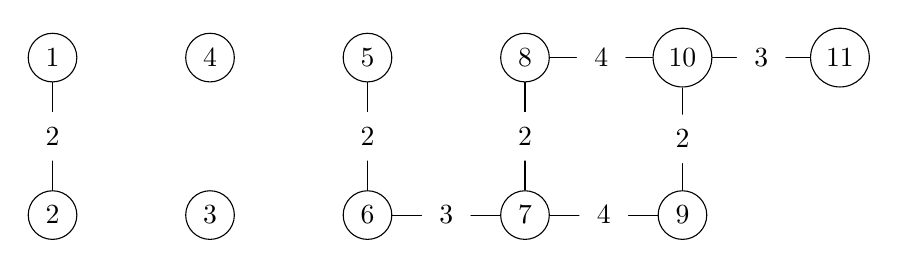
\begin{tikzpicture}

        \begin{scope}[every node/.style={circle,draw}]
          \node (1)  at (0,2)  {1};
          \node (2)  at (0,0)  {2};
          \node (3)  at (2,0)  {3};
          \node (4)  at (2,2)  {4};
          \node (5)  at (4,2)  {5};
          \node (6)  at (4,0)  {6};
          \node (7)  at (6,0)  {7};
          \node (8)  at (6,2)  {8};
          \node (9)  at (8,0)  {9};
          \node (10) at (8,2)  {10};
          \node (11) at (10,2) {11};
        \end{scope}

        \begin{scope}[every node/.style={fill=white,circle}]

          \begin{scope}[every edge/.style={draw}]
            \path (1)  edge node {$2$} (2);
            \path (5)  edge node {$2$} (6);
            \path (7)  edge node {$2$} (8);
            \path (9)  edge node {$2$} (10);
            \path (6)  edge node {$3$} (7);
            \path (10) edge node {$3$} (11);
            \path (7)  edge node {$4$} (9);
            \path (8)  edge node {$4$} (10);
          \end{scope}
        \end{scope}

      \end{tikzpicture}
      \caption{[1, 5, 994, 219, 381]}
    \end{center}
  \end{figure}

  \begin{figure}[H]
    \begin{center}
      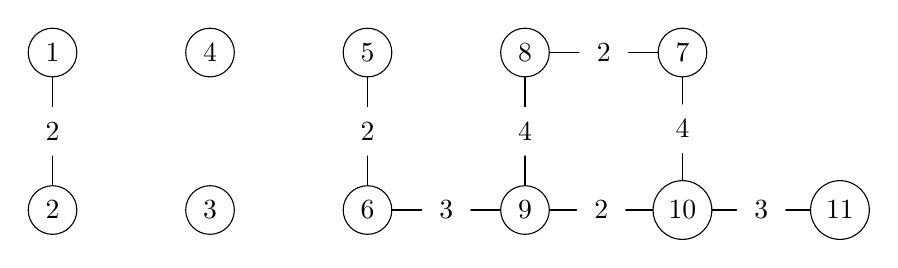
\begin{tikzpicture}

        \begin{scope}[every node/.style={circle,draw}]
          \node (1)  at (0,2)  {1};
          \node (2)  at (0,0)  {2};
          \node (3)  at (2,0)  {3};
          \node (4)  at (2,2)  {4};
          \node (5)  at (4,2)  {5};
          \node (6)  at (4,0)  {6};
          \node (7)  at (8,2)  {7};
          \node (8)  at (6,2)  {8};
          \node (9)  at (6,0)  {9};
          \node (10) at (8,0)  {10};
          \node (11) at (10,0) {11};
        \end{scope}

        \begin{scope}[every node/.style={fill=white,circle}]

          \begin{scope}[every edge/.style={draw}]
            \path (1)  edge node {$2$} (2);
            \path (5)  edge node {$2$} (6);
            \path (7)  edge node {$2$} (8);
            \path (9)  edge node {$2$} (10);
            \path (6)  edge node {$3$} (9);
            \path (10) edge node {$3$} (11);
            \path (7)  edge node {$4$} (10);
            \path (8)  edge node {$4$} (9);
          \end{scope}
        \end{scope}

      \end{tikzpicture}
      \caption{[1, 5, 994, 232, 267]}
    \end{center}
  \end{figure}

  \paragraph{}
  In all the graphs,

\end{proof}

\paragraph{}
Grâce à ces deux théorèmes, on sait qu'il existe une 2-transposition $g$ dont $\rho_2$ est une extension qui est telle que $ g \in \Gamma_{0,1} = S_7$ et $g \in \Gamma_(0,3,4)$ donc $g \in \Gamma_{0,1} \cap \Gamma_(0,3,4)$ mais $g \notin \Gamma_{0,1,3,4} = <\rho_2>$. Donc $\Gamma_{0,1} \cap \Gamma_{0,3,4} \neq \Gamma_{0,1,3,4}$ donc $\Gamma$ ne satisafait pas la propriété d'intersection et n'est donc pas un C-group. Ce qui conclut la preuve du théorème
